% chapter2 基础

\chapter{相关理论与技术}

\section{脑电生理基础}

\subsection{人脑结构与运动想象}

大脑作为神经活动的中枢处理器,其活动产生的多元生物电信号揭示了人体的认知行为、感官体验、情绪调控等多种思维活动和行动指令。通过现代神经科学技术,如脑电图、功能性磁共振成像、近红外光谱成像等手段,人类能够探测并解读这些生物信号,从而了解大脑内部的运作机制。

大脑皮层是大脑最外部的灰质结构,承载了复杂的高级认知功能。大脑皮层中与运动相关的结构主要包括初级运动皮层、辅助运动区、运动前区、顶叶皮层、前额叶皮层\cite{ZDYS201809014},此外,位于基底神经节的纹状体也参与其中。运动想象是一种心理活动,指的是在没有实际执行肢体运动的情况下,个体在脑海中模拟或重现某项运动的过程,研究发现,当个体执行运动想象任务时,即使没有运动执行,人脑中的相关脑区仍会呈现激活状态,其中,主要激活的是辅助运动区,辅助运动区在运动执行任务以及运动想象任务中与运动前区、感觉运动皮层区、默认网络结构都存在双向连接\cite{solodkin2004fine},并且存在指向纹状体的单向连接\cite{watanabe2015effects}。相对于运动执行任务,运动想象任务中主运动皮层也存在激活,但激活程度不及运动执行任务\cite{solodkin2004fine,kasess2008suppressive}。大脑皮层中各运动区的位置如图~\ref{fig:brain}~所示。
\begin{figure}[ht]
    \centering
    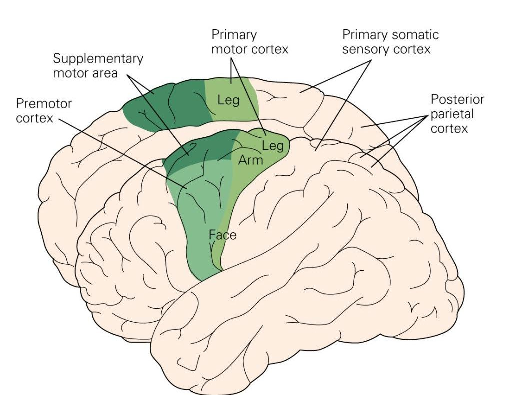
\includegraphics[width=0.3\textwidth]{brain.pdf}
    \caption{大脑皮层运动相关区域\cite{penfield1950cerebral}}
    \label{fig:brain}
\end{figure}

\subsection{脑电图信号及其特性}

脑电图信号由皮质内大量神经元突触后电位同步总和形成,是很多神经元共同活动的结果\cite{ZWQX201803022}。EEG信号可以分为深部EEG,皮层EEG和头皮EEG\cite{1022779250.nh}。相比深部EEG和皮层EEG,从头皮采集的EEG信号需穿透颅骨和头皮组织,因此具有相对较低的信号质量,但头皮EEG无需进行任何开创性手术,极大地降低了医疗风险,保证了高度的安全性,并且实施便捷,获取数据更为简易。因此,头皮EEG成为了神经系统疾病诊断、脑功能研究等领域广泛应用的首选工具。后文中所提到的EEG信号,如无特殊说明,都是指头皮EEG。

EEG信号使用脑电采集系统作为记录设备,其样式如图~\ref{fig:equip}~所示,通过在受试者头皮上放置单个或多个脑电极(或称通道),以连续、实时的方式记录一段时间内的大脑皮层产生的电信号。图~\ref{fig:montage}~展示了脑电极在头皮上的一种排列方式。EEG信号的采集方式决定了其数据的形状,通常为脑电极(通道)与时间构成的二维数据。对于单通道采集的数据,EEG信号可视化以电位为纵轴,时间为横轴,表示该通道上电位随时间的变化,图~\ref{fig:eeg}~为包含16个通道的EEG信号可视化,可视化中相邻的通道在空间上未必具有相邻关系。
\begin{figure}[ht]
    \centering
    \begin{subfigure}{0.3\textwidth}
      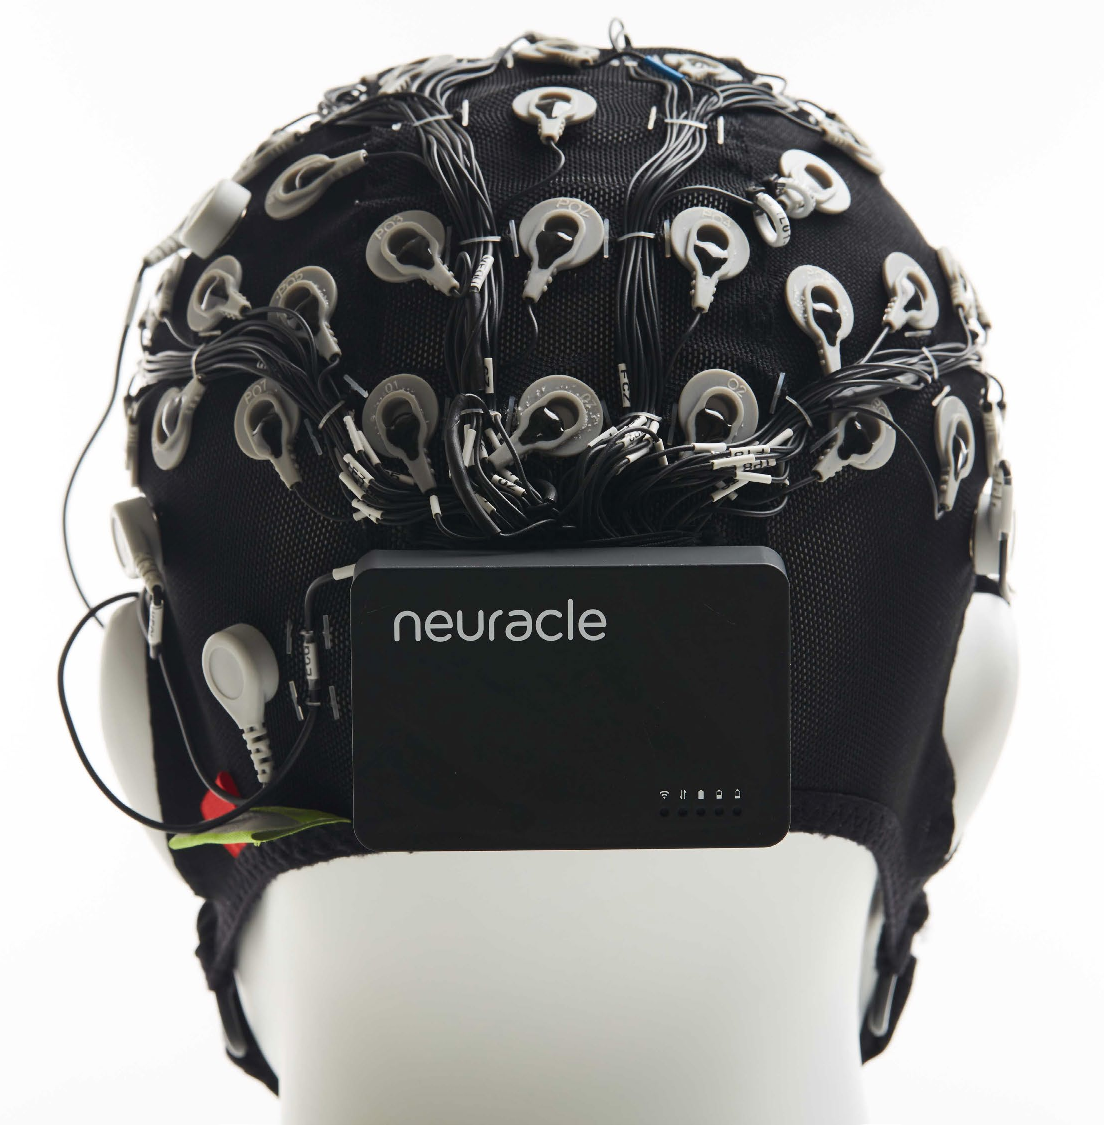
\includegraphics[width=\linewidth]{equip.pdf}
      \caption{脑电采集设备\cite{equip}}
      \label{fig:equip}
    \end{subfigure}\qquad
    \begin{subfigure}{0.3\textwidth}
      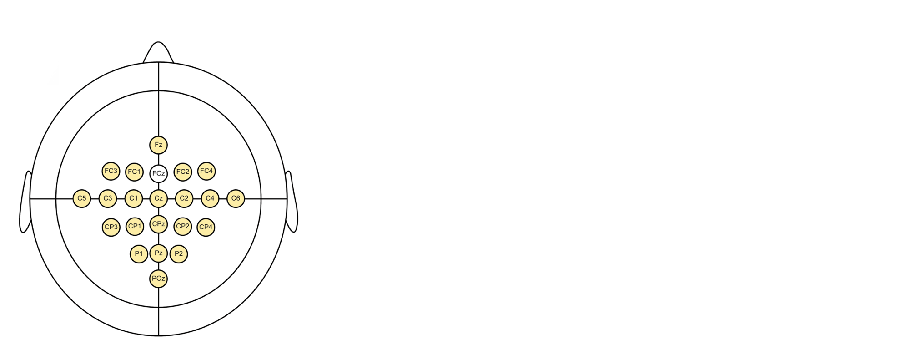
\includegraphics[width=\linewidth]{montage.pdf}
      \caption{一种脑电极排列方式\cite{han2023eeg}}
      \label{fig:montage}
    \end{subfigure}
    \caption{脑电信号采集}
    \label{fig:eeg-cap}
  \end{figure}
\begin{figure}
    \centering
    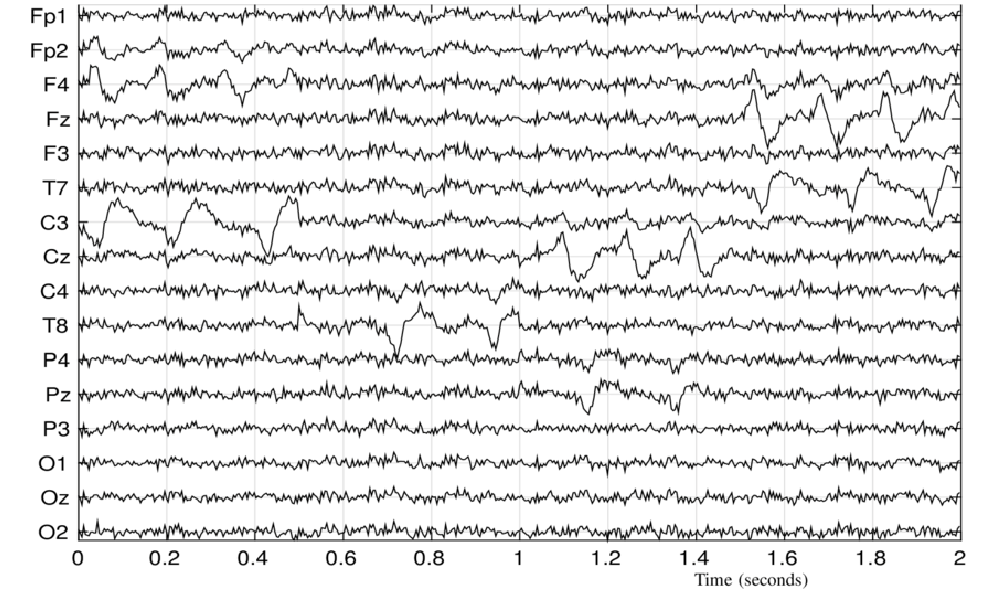
\includegraphics[width=0.5\textwidth]{eeg.pdf}
    \caption{EEG信号可视化}
    \label{fig:eeg}
\end{figure}

正常脑电信号是多个具有生物学意义的神经振荡节律的组合\cite{1022779250.nh}。神经科学研究发现,根据脑电信号的频率范围,能够划分出五种主要节律:

(1) Delta:频率范围为0.5-4Hz。研究发现,Delta波的起源主要有两个,分别是皮层和丘脑,后者主要与睡眠相关\cite{kropotov2010quantitative}。Delta节律主要出现在深度睡眠阶段,尤其是在儿童和婴儿的脑电图中尤为明显。成年人在某些病理状态下也可观察到增强的Delta节律,如严重的器质性脑疾病。

(2) Theta:频率范围为4-8Hz。Theta节律不仅出现在轻度睡眠和快速眼动睡眠阶段,还可见于青少年和儿童清醒时的脑电图中,以及成年人在专注、疲劳或焦虑状态下的头顶前部中线位置\cite{ishihara1966activation,ishihara1967interaction}。

(3) Alpha:频率范围为8-13Hz。Alpha节律依据起源位置的不同可分为两大类:一类是源自初级躯体感觉皮层的Mu节律(或称运动Alpha节律)\cite{hari1997human},手部运动、运动想象等活动可以阻断Mu节律,而在肌肉放松状态下则会增强Mu节律;另一类则是通常在个体放松、闭眼静息状态出现,来源于视觉皮层或枕叶的Alpha节律,其在睁眼或注意力集中时受到抑制,表现为振幅减小。此外,有研究指出,脑力劳动的增加也将导致Alpha节律活动的减弱\cite{1022779250.nh}。

(4) Beta:频率范围为13-30Hz。Beta节律根据分布区域的不同可分为两大类:一类是在感觉运动皮层区域表现最强的运动Beta节律,其活动强度受运动任务影响,在运动想象、运动准备和运动执行过程中,运动Beta节律的幅值功率都会有相应变化;另一类是在额叶区域表现最强的额叶Beta节律,此类节律主要出现在清醒、警觉、专注以及执行认知任务时的大脑活动中,其强度的增加通常与认知活动和心理负荷的上升相关联。

(5) Gamma:频率范围通常定义为超过30Hz,有时也指25Hz至100Hz甚至更高的频率范围。Gamma节律广泛参与到认知处理、意识维持、注意力集中、感知整合和记忆编码等复杂脑功能过程中,被认为与高级认知功能和信息整合紧密相关。Gamma节律可在多个脑区观察到,包括但不限于前额叶、顶叶和颞叶区域。

需要说明的是,各类脑电波的频率范围并不是绝对分割的,而是存在着一定的重叠与交织。在实际的大脑生理活动中,某一时刻或时间段内的脑电信号往往包含了多种不同的节律形态,不仅限于Delta、Theta、Alpha、Beta、Gamma五类,例如,运动Beta节律和额叶Beta节律可以同时出现。实际上,脑电极采集到的脑电信号通常是不同频率节律相互交织、叠加而成的复杂组合。

除却具有脑生理活动信息的EEG节律,脑电极会同时采集到各类噪声信息,称之为EEG伪迹。常见的EEG伪迹有以下几种:

(1) 眼动伪迹:当眼睛移动(如眨眼、扫视等)时,眼周的肌肉和眼睑的电位变化会在电极上产生强烈的电位波动。这种伪迹在额部电极附近特别明显,特征是突然出现的尖峰或方波形状的电位变化。眼动信号通过眼电图(Electrooculogram,EOG)记录。EOG的幅度一般是EEG信号的几倍,频率通常分布在3-16Hz,幅值通常分布在0.5-4mV。

(2) 肌电伪迹:肌电伪迹主要来自于头颈部及面部肌肉的伸展和收缩,如进行吞咽、呼吸、讲话等行动时,就会产生肌电伪迹。肌电伪迹通常表现为高频、大振幅的波动,与实际脑电活动相比更加剧烈和不稳定。肌电信号可以通过肌电图(Electromyogram,EMG)记录。EMG的频率在0-200Hz广泛分布。

(3) 心电伪迹:脑电极分布在脑部血管附近,心脏搏动会在头皮电极上产生明显的电位波动,尤其是在靠近耳朵后部的乳突区域。心电伪迹通常表现为周期性出现的正弦波形,与心脏搏动频率(大约每分钟60-100次)相符。心电信号可以通过心电图(Electrocardiogram,ECG)记录。ECG的波形类似EEG波形,频率在0.05-100Hz广泛分布。

(4) 工频伪迹:工频干扰来源于电源线和其他电气设备释放的50Hz(欧洲和亚洲大部分地区)或60Hz(北美和其他部分地区)的交流电噪声。这种干扰在EEG信号中表现为稳定的、与电源频率相同的周期性波动。

为了减少EEG信号中的伪迹干扰,通常会在数据预处理阶段运用一系列针对性算法和技术。例如,利用独立成分分析识别并排除源于眼动和肌电的伪迹成分,通过低通滤波抑制心电伪迹在特定频率范围内的影响等。然而,需要说明的是,即便是基于信号处理技术和神经科学先验知识,伪迹的去除过程仍有可能导致某种程度的真实脑电信息丢失。尤其是在处理复杂、微妙的脑电活动时,很难做到既能彻底清除伪迹又不损害有价值信号的完整性。

综上所述,EEG信号是一种蕴含丰富信息却又存在诸多问题的复杂生物电信号,它不仅涵盖着从Delta至Gamma等多种频率范围的脑电节律,且这些节律在实际记录中存在交错重叠的现象。此外,EEG信号容易受到多种噪声源的显著影响,包括眼动、肌电、心电伪迹等生理伪迹,工频干扰等非生理伪迹。鉴于EEG信号独特的生理特征和采集特点,它展现出一些鲜明的特性:

(1) 低信号强度。EEG信号采集的是神经元活动产生的微弱电压波动,其强度一般在\(\mu\)V级别(5-100\(\mu\)V)\cite{SJCJ201505001}。这使EEG信号易受噪声影响,提高了信号处理和解析的难度。

(2) 宽带特性,低信噪比。EEG信号所蕴含的有价值信息具有显著的时间动态性,即这些信息会随时间持续演变并在整个时间域内传播,这使得EEG信号在频谱分析中呈现出宽广的频率范围,其中包含的主要成分通常分布在大约0.5至45Hz的频率范围内\cite{1022779250.nh},涵盖了Delta、Theta、Alpha、Beta及部分Gamma节律。然而,由于伪迹噪声普遍存在且分布广泛,EEG信号中蕴含的有用信息时常与伪迹及其他信息在不同频带上相互交叉混叠。与此同时,由于人体脑电信号本身强度微弱,加之复杂的生理和心理状态变化,以及检测技术在实际应用中的不稳定性,进一步导致了在实际采集的EEG信号数据中,不同脑电成分之间易于互相干扰和混淆。这些现象显著降低了EEG信号的信噪比,即有用信号与噪声的比例较低。这为EEG信号的分析带来了困难,难以完整地将有用信号从背景噪声中剥离,并且需要依赖经验和神经科学先验知识,耗费相当的开销。

(3) 非平稳性,被试特异性。不同于平稳随机信号,EEG信号的统计特性随时间发生变化,其频率、幅度等特征在不同任务条件下呈现出显著的动态变化,表明EEG信号具有明显的非平稳性。与此同时,不同个体(被试)所产生的EEG信号在频率成分、幅度强度、响应时间等方面通常表现出个体间的差异性;不仅如此,即使是同一被试在不同时间段内执行同样的任务,其所产生的EEG信号也可能存在变化。因此,EEG信号具有显著的被试特异性,意味着每位被试的脑电活动模式在很大程度上是个体独有的。这使得很难使用一种固定的方法对EEG信号进行分析。

(4) 非线性。EEG信号不是单一过程的结果,而是多种脑内过程或同源过程非线性耦合与叠加的产物,呈现出显著的非线性特征。这种非线性特性使得各种信号成分之间的相互作用和影响更为复杂化,极大地提升了EEG信号分析的复杂度和难度。

(5) 多通道,时空分布不均。在实际采集过程中,EEG信号通常利用多个脑电极(通道)进行同步记录,形成了多通道数据属性。同时,EEG信号的时空分布不均匀,大脑在执行特定功能时,会在特定时间和脑区产生显著的电压波动,例如,进行眼球运动时,在额部电极附近会产生即时且明显的眼电活动。脑电极的分布通常使用国际10-20标准导联确定,其中,“10”和“20”指相邻电极之间的实际距离设定为头骨前后或左右总距离的10\%或20\%\cite{jasper1958ten},标准10-20导联系统包含了21个电极,这些电极捕获的信号在不同大脑活动中蕴含的信息量不尽相同。此外,EEG信号在时间域的数据量往往要高于空间域的数据量,且时间域蕴含的有效信息更为丰富。这种时空分布的不均衡性提升了筛选和提取有效信息的困难性。

EEG信号具有时间域、空间域、频率域三个维度的特征。在时间域层面,EEG信号揭示了神经活动随时间推移的动态变化过程;在空间域层面,EEG信号揭示了神经活动在不同头皮电极位置上的强度分布差异,反映了大脑不同区域的功能活动;而在频率域层面,EEG信号反映了信号中蕴含的不同脑电节律。脑电采集设备所采集到的原始EEG信号直观地反映了时间域和空间域的特征,如图~\ref{fig:eeg}~所示。频率域的特征则需要通过快速傅里叶变换等频谱分析技术对原始数据进行转换。相较于直接处理原始的EEG信号,提取频率域特征通常需要更多的计算资源和处理时间,耗费更高的开销。

\subsection{脑电图信号与运动想象}

事件相关去同步化(Event-Related Desynchronization,ERD)和事件相关同步化(Event-Related Synchronization,ERS)是在研究EEG信号过程中发现的两种脑活动现象,它们反映了大脑在特定任务或事件触发后,特定频段脑电活动的动态变化。

(1) 事件相关去同步:ERD是指在执行一项特定的任务,如运动想象或实际运动时,原本在一定频段上占主导地位的同步脑电活动(即电位振荡趋于一致)出现了减少或消失,表现为脑电功率的下降。这一现象通常与大脑皮层的兴奋性增加和特定区域活动增强有关。在运动想象或实际运动时,初级运动皮层和辅助运动区的Alpha节律(Mu节律)、Beta节律通常会出现ERD现象。

(2) 事件相关同步:ERS与ERD相反,是指在特定任务或事件发生后,某一频段的脑电活动同步性增强,表现为脑电功率的升高。ERS可能表示大脑某些区域的活动暂时减少或进入了一种休眠状态,为其他区域的活动让渡资源,或者代表了大脑在执行某些认知或精神任务时的资源重新配置。在运动想象或实际运动时,ERS现象会出现在Alpha节律(Mu节律)和Beta节律中。

在单侧肢体的运动想象中,大脑呈现出不对称的激活模式:对侧大脑半球(即与执行想象运动的肢体相对应的脑区)通常会出现更为显著的ERD现象,意味着该区域的特定频段脑电活动强度减弱\cite{pfurtscheller1977event}。与此同时,执行运动想象任务的同侧大脑半球则会出现一定程度的ERS现象。实际上,在运动想象任务结束后的放松阶段,ERS现象更为明显,此时大脑可能在先前活跃区域呈现出电活动同步性的增强,这一现象反映了大脑从运动想象状态向静息状态转变时的活动调整和资源分配。进行左右手运动想象时,脑功率谱密度变化如图~\ref{fig:erders}~所示,当想象左手运动时,大脑皮层右侧(C4电极附近)出现ERD现象,相关区域能量减小;当想象右手运动时,大脑皮层左侧(C3电极附近)出现ERD现象,相关区域能量减小\cite{blankertz2010neurophysiological}。
\begin{figure}[ht]
    \centering
    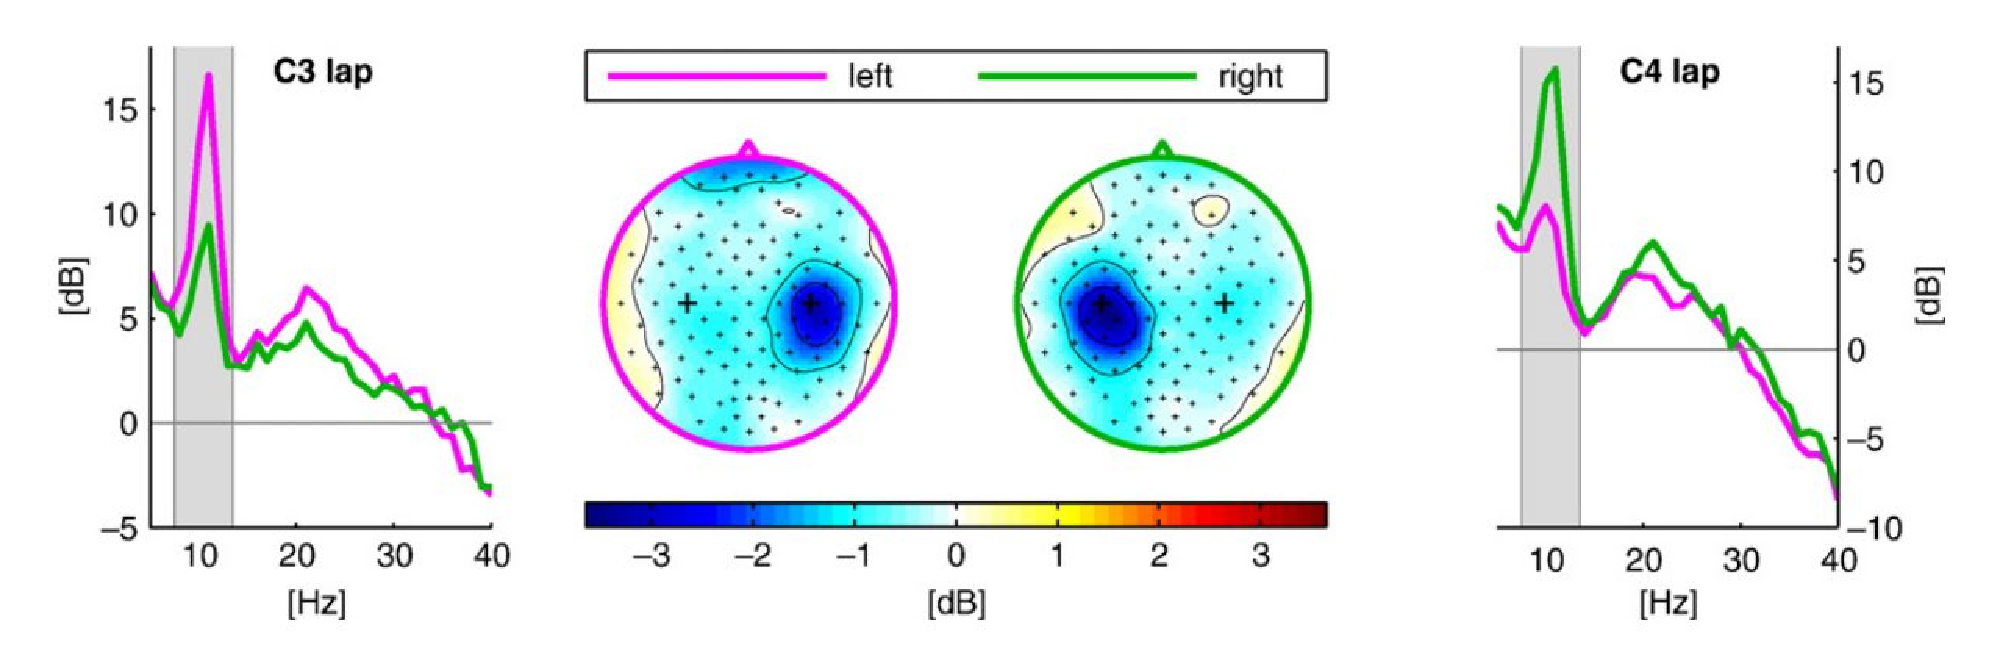
\includegraphics[width=0.9\textwidth]{erders.pdf}
    \caption{左右手运动想象的ERD现象\cite{blankertz2010neurophysiological}}
    \label{fig:erders}
\end{figure}

综上所述,与运动想象相关的脑电图信号主要是出现在感觉运动皮层的Mu节律和Beta节律,进行运动想象时,主要会出现ERD、ERS这两种脑电活动现象。

\section{深度神经网络基础}

深度神经网络(Deep Neural Network,DNN)是一种基于对人脑的模拟设计的多层非线性模型,在计算机视觉、自然语言处理、语音交互等领域有着广泛的应用。相较于传统的神经网络,深度神经网络通过多个隐藏层逐层对输入数据进行特征提取和抽象,模型的复杂性和表达能力实现了大幅的提升,能够对更复杂的非线性关系进行拟合,取得更为优异的性能和效果。

\subsection{卷积神经网络}

卷积神经网络是深度学习领域经典且重要的模型,其设计灵感来自于生物学中对动物视觉系统的理解,设计目的是模拟人类的视觉处理过程。CNN在计算机视觉领域取得了巨大成功,广泛应用于图像识别、图像分类、物体检测、语义分割、视频分析等任务中,其优势在于能够自动学习图像特征,无需进行人工特征提取,从而简化了流程,并提高了性能。

CNN的结构主要包括输入层(Input Layer)、卷积层(Convolutional Layer)、池化层(Pooling Layer)、激活函数(Activation Function)、全连接层(Fully Connected Layer)、输出层(Output Layer),此外还可包括Dropout层、归一化层(Normalization Layer)等。一个简单的用于分类任务的CNN网络结构如图~\ref{fig:cnn}~所示。论文将对其中的重要结构进行说明。
\begin{figure}[ht]
    \centering
    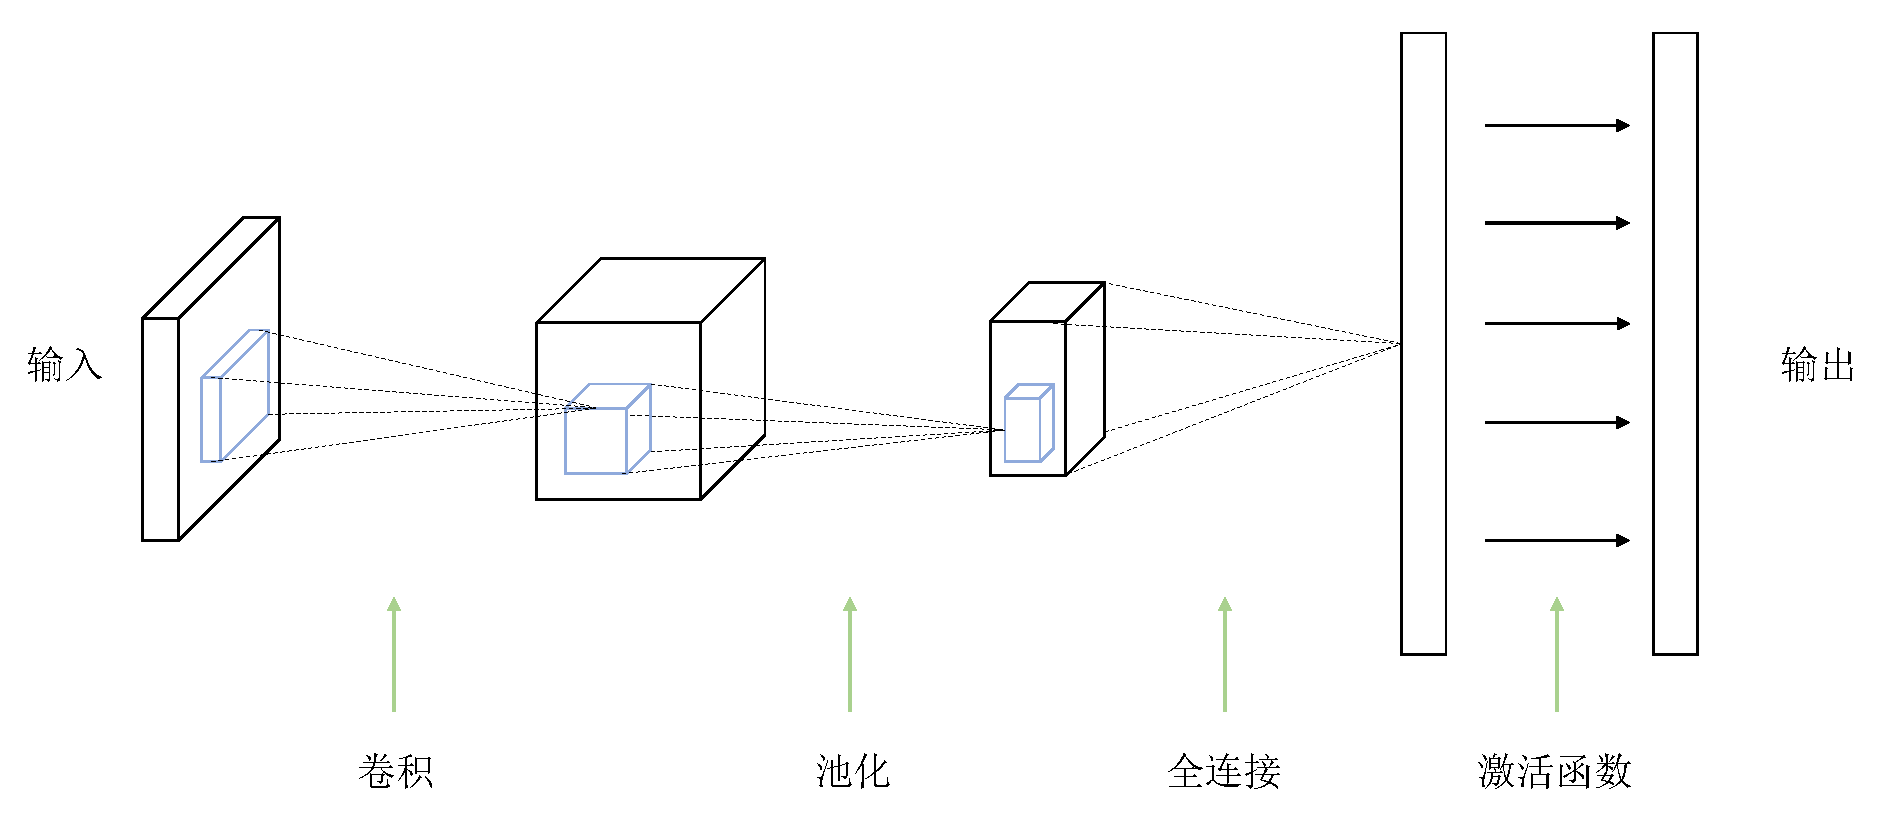
\includegraphics[width=0.6\textwidth]{cnn.pdf}
    \caption{多分类卷积神经网络基本结构}
    \label{fig:cnn}
\end{figure}

\paragraph{卷积层}

卷积层是CNN的核心组成部分之一,它对人类视觉系统中的感受野(Receptive Field)进行模拟,对图像的局部特征进行提取。卷积层使用一组可学习的滤波器(Filter),或称卷积核(Kernel)在输入数据上进行滑动,并与覆盖窗口内的数据做元素间乘法和加法运算,得到一个特征图(Feature Map)或激活图(Activation Map),这种计算过程被称为卷积。卷积操作中有许多可设置的参数,如卷积核的大小(Kernel Size),卷积核滑动的步长(Stride),数据填充(Padding)等。卷积核的大小决定了局部感受野的大小,较大的卷积核可以捕获更大范围的上下文信息,而较小的卷积核在捕获局部细节上更具优势;步长决定了卷积核在数据上移动的间距,当步长为1时,进行逐元素的卷积;填充是在数据外缘填充额外的数据,一般用于对数据大小进行扩充,使得卷积后能够获得与原数据大小相同的特征图。图~\ref{fig:conv}~展示了在一个\(4\times4\)的输入数据上进行卷积的过程,卷积核大小为\(3\times3\),步长为1,填充为1。
\begin{figure}[ht]
    \centering
    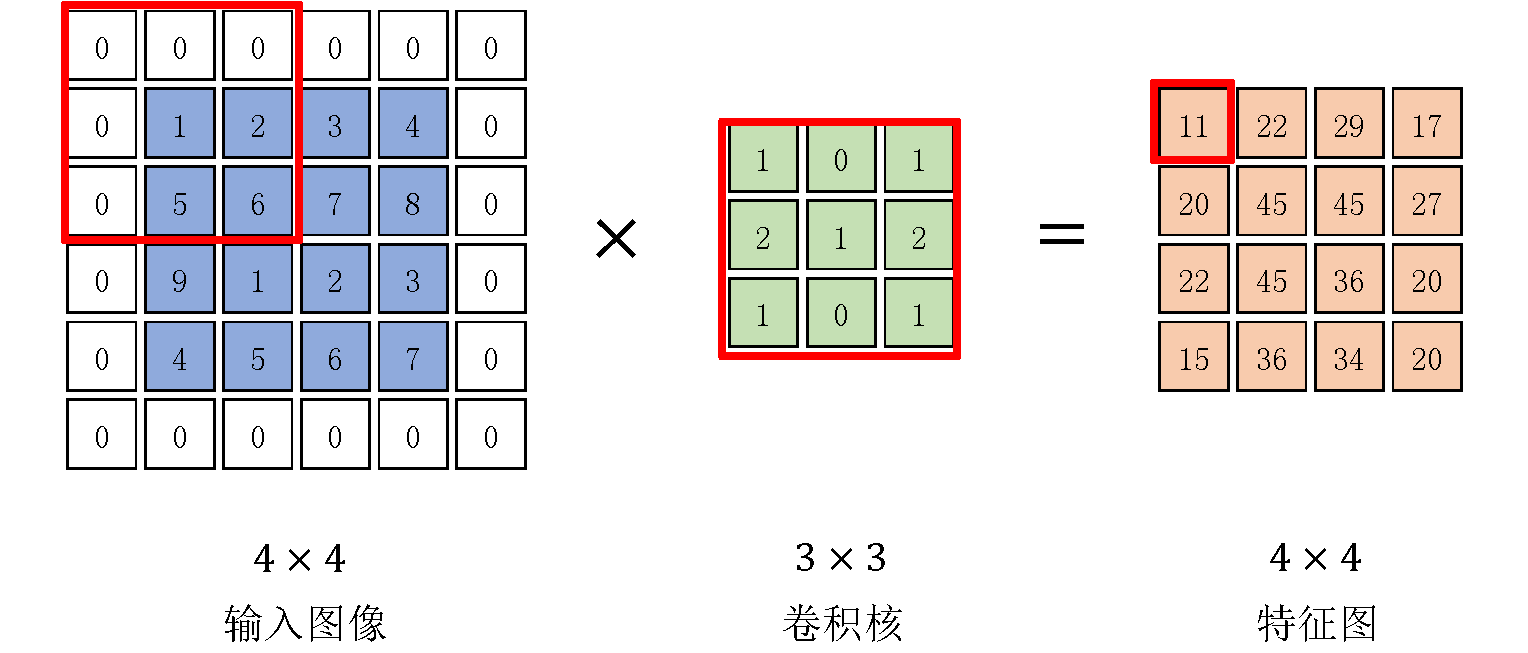
\includegraphics[width=0.6\textwidth]{conv.pdf}
    \caption{二维卷积运算}
    \label{fig:conv}
\end{figure}

在处理如彩色图像这类多通道数据时(如RGB三通道),卷积核的通道数与输入图像的通道数相匹配,卷积核的每个通道分别与输入图像的相应通道进行卷积操作,然后将各个通道的结果进行逐元素相加,形成最终的输出特征图,其过程如图~\ref{fig:mutconv}~所示,其中使用了一个具有三通道的卷积核。
\begin{figure}[ht]
    \centering
    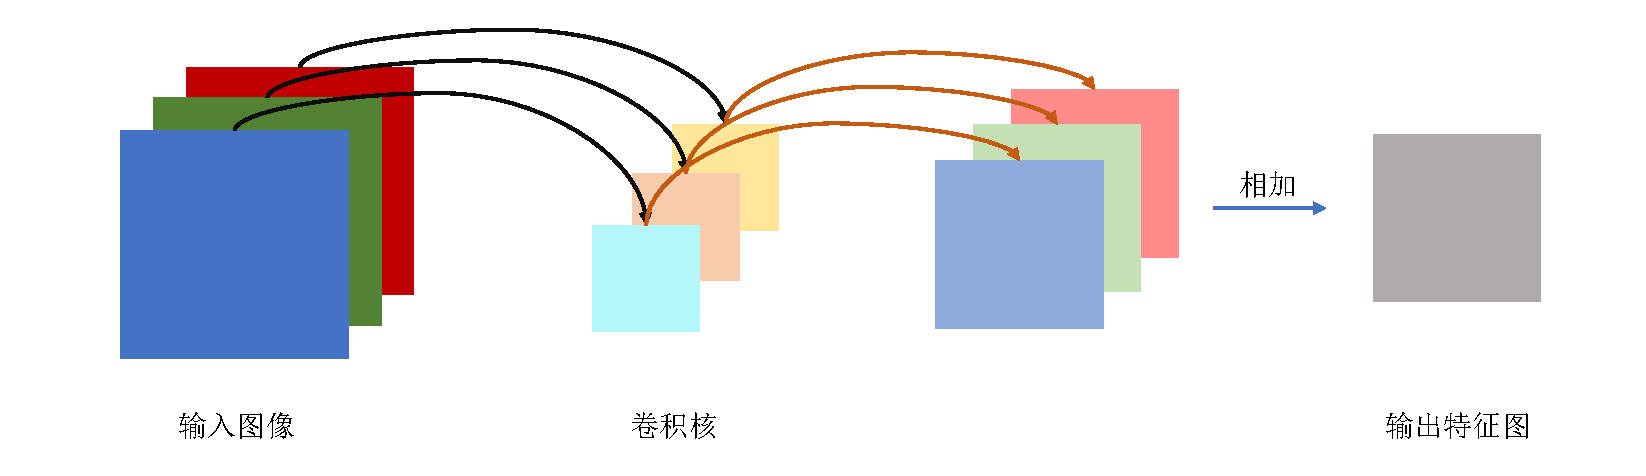
\includegraphics[width=0.6\textwidth]{mutconv.pdf}
    \caption{多通道卷积运算}
    \label{fig:mutconv}
\end{figure}

在经过卷积操作生成的特征图中,任一元素实质上是由上一层特征图中的\(N \times N\)个相邻元素加权组合而成,使得该元素具有\(N \times N\)大小的感受野。随着卷积层的叠加,感受野逐渐扩大,意味着在深层的特征图中,一个元素能够捕获到输入中更广阔区域的信息,提取到的特征更为高级和抽象。图~\ref{fig:highconv}~展示了感受野随层次加深的变化。
\begin{figure}[ht]
    \centering
    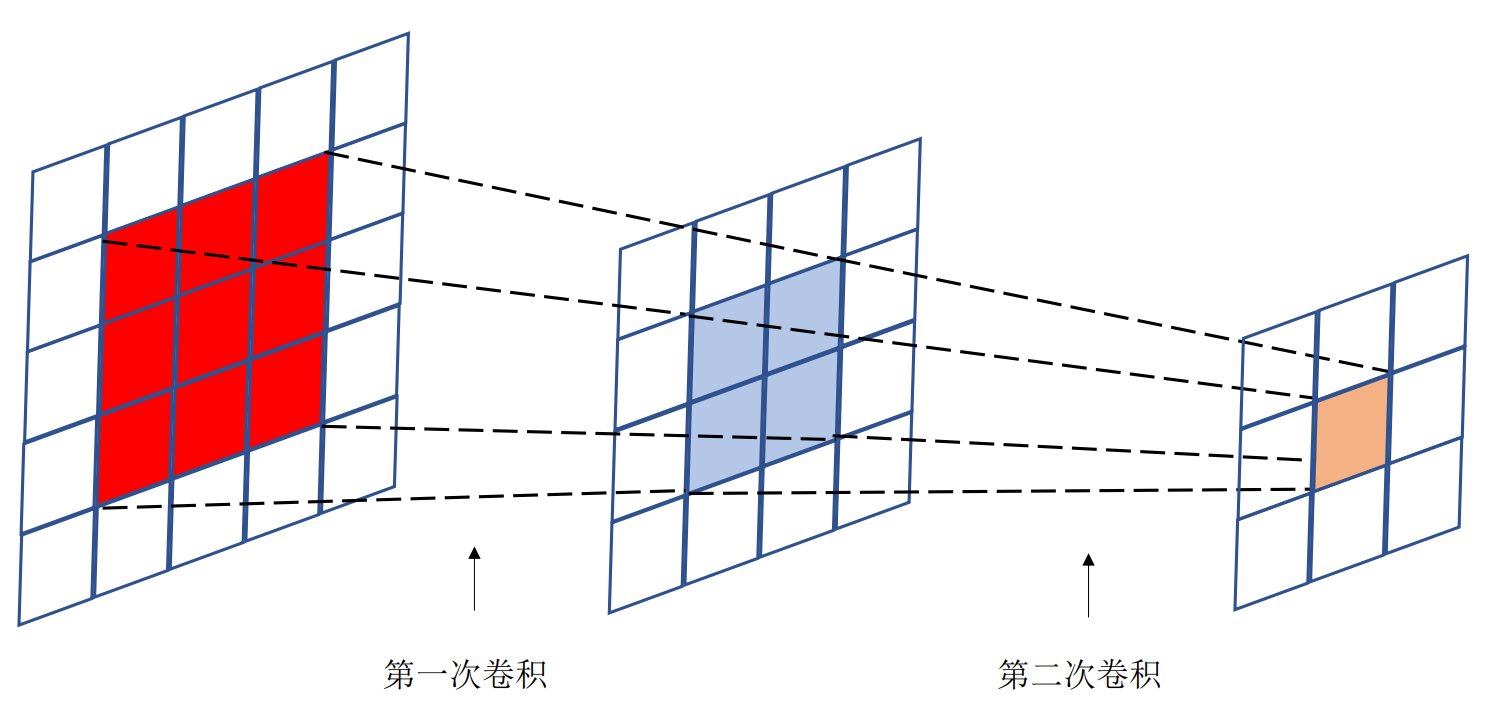
\includegraphics[width=0.5\textwidth]{highconv.png}
    \caption{感受野随层次加深示例}
    \label{fig:highconv}
\end{figure}

\paragraph{池化层}

池化层是CNN的重要组成部分之一,用来对特征图进行降维,从而在保留重要信息的同时减少参数的数量。池化层的主要类型为最大池化(Max Pooling)和平均池化(Average Pooling),此外还有最小池化(Minimum Pooling)、L2范数池化(L2-Normalized Pooling)等,但在实际应用中并不常见。

在最大池化中,池化层将输入特征图中每个区域的最大值作为输出,能够保留特征图中最为明显的特征;在平均池化中,池化层将输入特征图中每个区域的平均值作为输出,相较于最大池化,平均池化更为平滑,能够降低特征图中的噪声,但可能会丢失一些细节信息。池化层中的可调参数通常是池化核的大小和步长,池化核的大小决定了池化操作所覆盖的局部区域的大小,步长决定了池化核每次移动的距离,二者共同决定了输出特征图的空间维度。图~\ref{fig:pooling}~展示了最大池化和最小池化的计算过程,其中,池化核的大小都为\(2\times2\),步长都为1。在CNN中,池化层通常与卷积层交替堆叠,构成特征提取的基本结构。
\begin{figure}[ht]
    \centering
    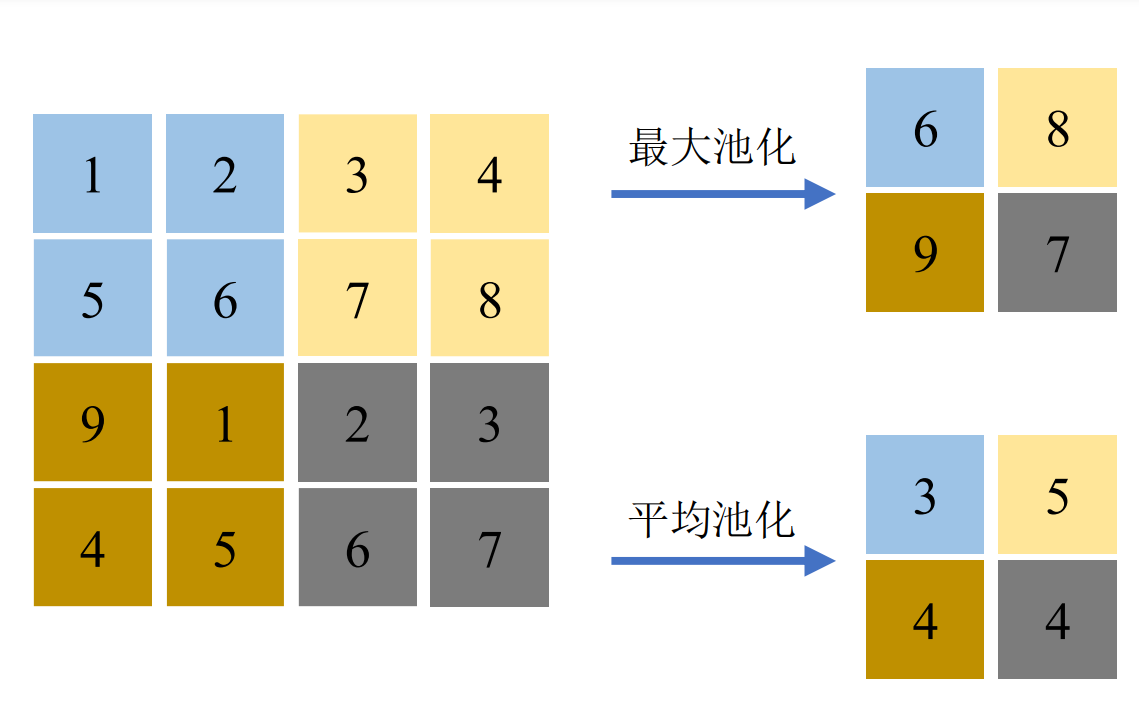
\includegraphics[width=0.4\textwidth]{pooling.png}
    \caption{最大池化与平均池化}
    \label{fig:pooling}
\end{figure}

\paragraph{激活函数}

激活函数是神经网络中的一种非线性函数,它对神经元的输出进行非线性变换,使得神经网络能够学习和表示更加复杂的函数关系。常用的激活函数有以下几种:

a. Sigmoid函数:Sigmoid函数将输入信号映射\((0,\,1)\)范围,其特点为平滑、连续、连续可微等,常用于二分类任务中。其公式为:
\begin{equation}
    Sigmoid(x) = \frac{1}{1 + e^{-x}}
    \label{eq:sigmoid}
\end{equation}
Sigmoid函数的缺点在于:当输入较大或较小时,Sigmoid的导数趋近于0,导致反向传播时神经元的权重难以更新,容易出现梯度消失现象;Sigmoid的输出不以0为中心,导致收敛速度变慢;函数中的指数级运算使得计算成本较高。

b. Softmax函数:Softmax函数将输入映射至\((0,\,1)\)区间,并且使得它们的总和为1,具有平移不变性、对数凸函数等特点,常用于多分类任务中。其公式为:
\begin{equation}
    Softmax(x_i) = \frac{e^{x_i}}{\sum_{j=1}^{N} e^{x_j}}
    \label{eq:softmax}
\end{equation}
其中,\(x_i\)是输入中的一个元素,\(N\)是输入的维度。Softmax函数的缺点在于,当某个类别的预测概率接近1时,对应的梯度几乎为0,使得梯度下降缓慢,出现梯度饱和现象等。

c. ReLU函数\cite{glorot2011proceedings}:ReLU函数将负数映射为0,正数保持不变,具有运算简单、收敛迅速的特点,在主流模型中应用广泛。其公式为:
\begin{equation}
    ReLU(x) = \max(0, x)
    \label{eq:relu}
\end{equation}
ReLU函数的缺点在于,在输入为负值时,ReLU的导数恒为0,导致部分神经元无法更新参数,出现神经元坏死现象。

d. GELU函数\cite{hendrycks2016gaussian}:GELU函数是一种基于高斯分布的激活函数,主要目标在于结合ReLU函数及其变种的优点,同时避免其中存在的一些问题,例如ReLU函数的神经元坏死,Sigmoid函数的梯度消失现象等。GELU的公式定义为:
\begin{equation}
    GELU(x) = x\Phi(x)
    \label{eq:gelu1}
\end{equation}
其中,\(P(X \le x)\)表示\(x\)的高斯正态分布的累计分布函数,由于计算困难,一般使用公式进行近似计算。
\begin{equation}
    GELU(x) = \frac{1}{2}x\left(1 + \tanh\left(\sqrt{\frac{2}{\pi}} \cdot \left(x + 0.044715x^3\right)\right)\right)
    \label{eq:gelu2}
\end{equation}
GELU的优点在于:具有更为光滑的导数,使得梯度可以更容易地进行传播,避免了零点导数不连续的问题,有助于解决梯度消失和梯度爆炸的现象;保持了ReLU在正数的线性增长特性,同时在负数也有非零梯度,解决了ReLU的神经元坏死现象;基于自然分布提出,能够更好地对人脑神经元进行模拟。鉴于这些优点,GELU函数当前在越来越多的模型中得到应用,如无特殊说明,论文使用的激活函数都是GELU函数。

\paragraph{归一化层}

归一化层是CNN的常见组成部分,能够减少因数据分布的变化而带来的内部协变量偏移、梯度消失、梯度爆炸等问题,用于提升训练的稳定性、加速收敛以及增强模型的泛化能力。常见的归一化层有以下三种:

a. 批量归一化(Batch Normalization,BN):BN对每一层神经网络的输入按批次(Batch)进行归一化,即对每个批次内的每一个特征图(通道)分别计算其均值和方差,然后对数据进行归一化,最后可以通过两个可学习的参数\(\gamma\)和\(\beta\)进行缩放和平移,以恢复数据的表达能力。BN将输入数据的分布调整为均值为0,方差为1的标准正态分布。BN具有一定的正则化效果,可以减少对Dropout层的依赖。

b. 层归一化(Layer Normalization,LN):不同于BN对整个批次进行归一化,LN是对单个样本的同一层的所有神经元的输出进行归一化,特别适用于循环神经网络之类用以处理序列数据的模型,在使用小批量数据进行训练时也可以有效应用。

c. 组归一化(Group Normalization,GN):GN通常与分组卷积\cite{krizhevsky2017imagenet}一起使用,将特征图(通道)分为若干组,对每一组内的神经元输出进行归一化。GN兼顾了BN和LN的优点,在小批量数据训练等场景具有良好的性能。

\paragraph{Dropout层}

Dropout是一种正则化技术,主要用于缓解神经网络在训练过程中可能产生的过拟合现象。Dropout的思想在于,通过在训练过程中随机地将一些神经元的输出“丢弃”,促使各神经元独立学习特征,减少相互的依赖。运算过程中,Dropout为每个神经元分配一个保留概率\(p\),表明其输出被纳入后续计算的概率。在每次迭代中,为了保持整体的期望输出不变,随机选择一些神经元,将它们的输出以\(p\)的概率丢弃,并将其余神经元的输出值除以\(1-p\)。进入测试阶段,Dropout调整为保持所有神经元的输出,并对它们的输出统一乘以\(p\),确保模型的期望输出与训练时的相符,无需继续进行随机丢弃。

\subsection{循环神经网络}

循环神经网络是一种用于处理序列数据的深度神经网络结构,其内部的循环连接使得网络在处理每个时间步的输入时都能够保留之前的信息状态,即具有“记忆”能力。这种特性使得RNN特别适合用来处理具有先后顺序的数据,如时间序列数据、自然语言文本等。

原始的RNN模型中的循环连接使得梯度在进行传播时容易呈现指数级衰减或增长的问题,即容易出现梯度消失或梯度爆炸现象,从而导致模型难以训练,难以捕捉到序列数据中的长期依赖关系。长短期记忆网络针对这些问题进行了改进,成为现阶段被广泛使用的基于RNN架构的模型之一。LSTM引入了门控机制,通过一系列门控单元控制信息的存储、读取和更新,从而实现对长期和短期信息的有效管理。LSTM的主要组成部分包括单元状态(Cell State)、遗忘门(Forget Gate)、输入门(Input Gate)和输出门(Output Gate),LSTM一个元胞的结构如图~\ref{fig:lstm}~所示,其中,\(h_{t-1}\)表示前一时间步的隐藏状态,\(c_{t-1}\)表示前一步的单元状态,\(x_t\)表示当前时间步的输出,\(f_t\)表示忘记门,\(i_t\)表示输入门,\(o_t\)表示输出门,\(\sigma\)为Sigmoid激活函数,代表门控的程度,\(tanh\)为双曲正切激活函数,用于更新细胞状态。多个元胞前后相连,就组成了LSTM。
\begin{figure}[ht]
    \centering
    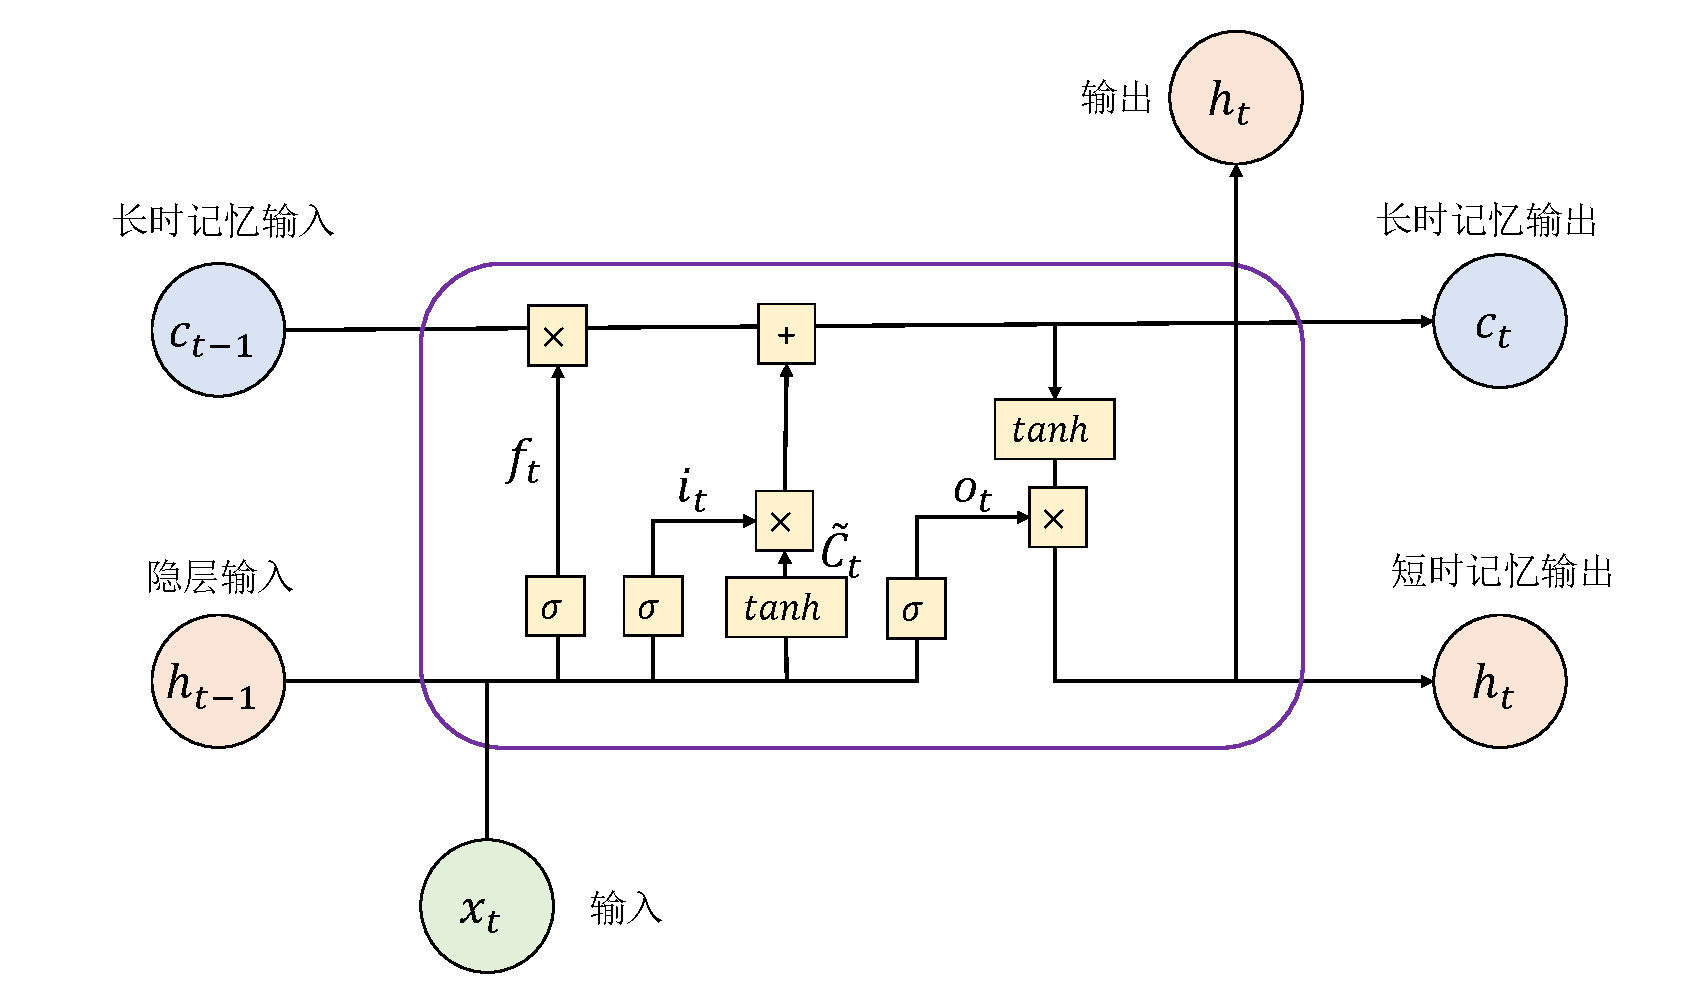
\includegraphics[width=0.6\textwidth]{lstm.pdf}
    \caption{LSTM元胞结构}
    \label{fig:lstm}
\end{figure}

\paragraph{单元状态}

单元状态用于存储和传递序列数据中的长期依赖信息,其通过遗忘门、输入门和输出门的控制,来决定如何更新和传递记忆信息。更新单元状态的公式如公式~\ref{eq:cell}~所示。
\begin{equation}
    c_t = f_t \odot c_{t-1} + i_t \odot \tilde{c}_t
    \label{eq:cell}
\end{equation}
其中,\(\odot\)表示逐元素相乘的Hadamard乘法,\(\tilde{C}_t\)表示候选单元状态,其计算方式如公式~\ref{eq:cell1}~所示,其中,\(W_c\)是用于单元状态更新的权重参数,\(b_c\)是偏置参数。
\begin{equation}
    \tilde{c}_t = \tanh(W_c \cdot [h_{t-1}, x_t] + b_c)
    \label{eq:cell1}
\end{equation}

\paragraph{遗忘门}

遗忘门用于控制哪些信息应当从单元状态中“遗忘”。遗忘门的输出值在0和1之间,代表每个单元状态中的信息应该被保留或遗忘的程度,其计算过程如公式~\ref{eq:forget}~所示,
\begin{equation}
    f_t = \sigma(W_f \cdot [h_{t-1}, x_t] + b_f)
    \label{eq:forget}
\end{equation}
其中,\(W_f\)是遗忘门的权重参数,\(b_f\)是偏置量。

\paragraph{输入门}

输入门用于控制哪些新信息应当被“记住”。输入门决定了候选单元状态被记忆的程度,即有多少信息被加入单元状态中。输入门的计算如公式~\ref{eq:in}~所示,
\begin{equation}
    i_t = \sigma(W_i \cdot [h_{t-1}, x_t] + b_i)
    \label{eq:in}
\end{equation}
其中,\(W_i\)是输入门的权重参数,\(b_i\)是偏置量。

\paragraph{输出门}

输出门用于控制从单元状态传递到当前时间步的隐藏状态(Hidden State)的信息量,输出门的计算如公式所示,
\begin{equation}
    o_t = \sigma(W_o \cdot [h_{t-1}, x_t] + b_o)
    \label{eq:out}
\end{equation}
其中,\(W_o\)是输出门的权重参数,\(b_o\)是偏置量。

\paragraph{隐藏状态}

隐藏状态(Hidden State)用于捕捉序列数据中的信息和特征,并传递给下一个时间步或输出层。隐藏状态通过循环连接获取上一个时间步的隐藏状态,能够存储序列数据中的历史信息,其计算过程如公式~\ref{eq:hs}~所示。
\begin{equation}
    h_t = o_t \cdot \tanh(c_t)
    \label{eq:hs}
\end{equation}

\subsection{注意力机制}

注意力机制(Attention Mechanisms)的提出受到人类认知科学的启发,其核心理念在于模拟人类大脑在处理信息过程中的选择性关注机制,即并非均匀地分配注意力处理对待所有输入,而是将注意力主动、动态且有选择性地聚焦于最重要或最相关的信息上。自二十世纪被提出以来\cite{730558},注意力机制在计算机视觉、自然语言处理等领域得到了广泛的应用,并表现出了优秀的效果。

注意力机制的基本思想为计算每个位置的权重,代表该位置对输出的重要性,权重通常可以由可学习的函数或神经网络生成,是一个与输入相同大小的矩阵,使用权重对输入数据进行加权操作,从而为重要的数据分配更多的关注。注意力机制通常包括查询矩阵(Query)、键矩阵(Key)和值矩阵(Value),其计算如公式~\ref{eq:sa}~所示,
\begin{equation}\label{eq:sa}
    Attention(Q,\,K,\,V)=softmax(\frac{QK^{T}}{\sqrt{d_k}}V)
\end{equation}
其中,\(Q\)为查询矩阵,\(K\)为键矩阵,\(V\)为值矩阵,\(d_k\)为键的维度。输入数据首先通过查询、键和值三个矩阵进行变换,然后计算出每个位置的注意力得分(Attention Score),这个得分衡量了数据中每个位置与当前处理位置之间的关联强度,所有位置的得分构成注意力矩阵。接着,使用Softmax函数获取注意力矩阵的归一化表示,最后,使用注意力矩阵对输入数据进行加权求和,从而得到最终的结果。注意力机制的结构如图~\ref{fig:sa}~所示。
\begin{figure}[ht]
    \centering
    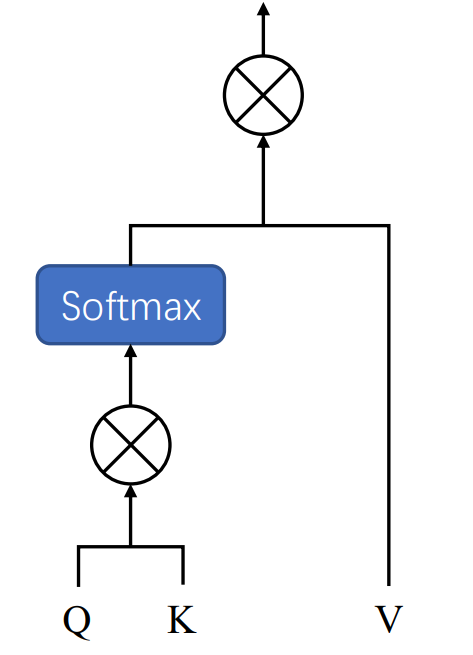
\includegraphics[width=0.2\textwidth]{sa.png}
    \caption{注意力机制}
    \label{fig:sa}
\end{figure}

注意力机制有多种变体,其中最常见的是点积注意力(Dot-Product Attention)和加性注意力(Additive Attention)。点积注意力使用输入序列和当前输出的点积来计算注意力权重,而加性注意力则使用一个全连接神经网络来学习权重。此外,还有自注意力\cite{vaswani2017attention}(Self Attention)机制,其计算每个位置上的元素与序列中所有其他元素的相关性来动态获取上下文信息,以捕获序列内部的依赖关系。

\section{本章小结}

本章主要介绍了与论文研究工作相关的理论和方法。首先,介绍了运动想象脑电图分类相关的生理基础知识,包括运动想象与人脑神经系统的关系、脑电图信号及其特性,为论文后续的研究进行铺垫。其次,论文介绍了深度神经网络的一些理论和模型,包括卷积神经网络、循环神经网络和注意力机制,也是论文后续研究中会用到的方法。通过本章内容,能够了解运动想象脑电图分类和深度神经网络的基础知识和常用方法,为后续的研究和应用奠定基础。